\section{Message from the Program Committee Co-Chairs}\vspace{2em}
\setheaders%
    {Message from the Program Committee Co-Chairs}%
    {Message from the Program Committee Co-Chairs}
\thispagestyle{emptyheader}
%\renewcommand{\large}{\fontsize{9}{11}\selectfont}
% that's a hack to make this part nicely fill the pages

\setlength{\parskip}{.7ex}
%\setlength{\parindent}{0pt}


Welcome to the 56th Annual Meeting of the Association for Computational Linguistics 2018 -- or ACL 2018 for short. 

In September 2017, Program Committee Co-Chairs (PCs) posted the call for nominations of Area Chairs (AC), Reviewers and Invited Speakers. We received 752 responses in total. Overall, out of 388 valid nominations for area chairs, 299 unique persons were suggested; 110 persons were self-nominations. About 70\% of the 56 selected area chairs (later expanded to 61 area chairs due to the high number of submissions) were nominated by the community. For the reviewers, we collected 936 valid nominations. At the PhD level, 139 persons were self-nominations and 129 were nominated by others. At the Postdoc/Ass.Prof.~level, 160 were self-nominated, 112 nominated by others. At the Prof.~level, 221 persons were self-nominated, 175 nominated by others. 

We received 138 unique nominations for invited speakers, from which two invited speakers of the conference were selected: 
\begin{itemize}
	\item Carolyn Penstein Rosé, Language Technologies Institute at Carnegie Mellon University, USA
	\item Anton van den Hengel, Australian Centre for Visual Technologies at University of Adelaide, Australia
\end{itemize}

%% # reviewers: 1473 (primary), 137 (secondary) -> total 1610
%% # good reviewers: 192

Our community is steadily growing: in total, 1621 submissions were received right after the submission deadline: 1045 long, 576 short papers. 13 erroneous submissions were deleted or withdrawn in the preliminary checks by PCs. 25 papers were rejected without review (16 long, 9 short); the reasons are the violation of the ACL 2018 style and dual submission guidelines. 32 papers were withdrawn before the review period started; the main reason was that the papers have been accepted as the short papers at NAACL HLT 2018. In total, 1551 papers went into the reviewing phase: 1021 long, 530 short papers. 1610 reviewers (1473 primary and 137 secondary reviewers) were involved in the reviewing process; each reviewer has reviewed about 3 papers on average.  3 long and 4 short papers were withdrawn during the reviewing period, and finally 1018 long and 526 short papers were considered during the acceptance decision phase.

The assignment of papers to areas and reviewers has been done in multiple rounds. First round: Initial assignments of papers to areas were determined automatically with the help of the authors’ input, while PCs went through all submissions and moved papers to other areas, considering COI and the topical fit. PCs assigned one AC as a meta-reviewer to each paper using Toronto Paper Matching System (TPMS) scores. Second round: ACs looked into the papers in their area, and adjusted meta-reviewer assignments. ACs sent a report to PCs if they found any problems. Third round: PCs made the final decision, considering the workload balance, possible COIs and the topical fit. Fourth round: ACs decided which reviewers would review each paper, based on AC’s knowledge about the reviewers, TPMS scores, reviewers’ bids, and COI.

We have introduced several innovations to the reviewing process. One of them is an argument-based review form. The reviewers were asked to provide arguments for and against the paper. This has been tremendously helpful for ACs and PCs to analyze the reviews and come up with final recommendations. The authors were asked to respond to the con arguments during the rebuttal. In coordination with the NAACL HLT 2018 PCs, we plan to do some analytics on anonymized reviews and rebuttal statements, with the consent of the reviewers and authors. Our purpose is to improve the quality of the review process. The data will be compiled into a unique corpus for NLP, and will be made available to the research community after appropriate anonymization checks, at the earliest in 2 years after ACL 2018. We hope to provide data on \emph{how to review} to younger researchers, and to improve the transparency of the reviewing process in general. 

The ACL 2018 conference is super-competitive: We accepted 256 out of 1018 submitted long papers and 125 out of 526 short papers, with an overall acceptance rate of 24.7\%. The details of the review process are available at the conference homepage. 
Criteria of acceptance were mainly: 
\begin{itemize}
	\item strengths/weaknesses raised by reviewers and their significance;
	\item the result of discussions and author responses;
	\item contribution to CL as the science of language: whether the paper advances (or contributes to) our understanding of language in any way;
	\item diversity: we do not want to fill ACL with similar papers like achieving 1\% improvement on a well-known task.  
\end{itemize}
We also considered the balance of paper types, topics and contributions and
re-considered the acceptance when reviewers reported any problem in preliminary checks (\textit{Appropriateness} to \textit{Handling of Human Participants}).

Continuing the tradition, ACL 2018 will feature 20 papers
which were accepted for publication in the Transactions of the
Association for Computational Linguistics (TACL). The TACL papers
were split into 10 oral presentations and 10 poster presentations.

There are many people to thank for who have worked diligently to
make ACL 2018 possible. All names are listed in the Program Committee section of the Front
Matter. 

Since the conference size continues to grow and the organizational complexity increases, we have introduced the role of Program Committee Co-Chair Assistants. In total, 5 senior researchers have supported the PCs during most intensive work phases to handle the communication in a timely manner, draft various documents and effectively prepare decisions.

Thanks to our area chairs for their hard work on recruiting reviewers, managing reviews,
leading discussions, and making recommendations.  

This program certainly would not be possible without the help of
the 1610 reviewers.
%Their names are listed in the Program Committee section.  
In particular, 192 reviewers from this list were recognized
by the area chairs as outstanding reviewers who have turned in exceptionally
well-written and constructive reviews and who have actively engaged themselves in
the post-rebuttal discussions. 

We are also deeply indebted to the best paper selection committee which consists
of 22 members. They had to additionally review 6-8 papers according to the best paper criteria on short notice. Their time and effort in recommending the best paper awards is much appreciated.

We also would like to thank many colleagues for generously sharing their experience in
organizing prior ACL conferences and for their advice. We are
grateful for the guidance and the support of the ACL presidents
Joakim Nivre and Marti Hearst, and the ACL board. We also would like to thank
the publication co-chairs Shay Cohen, Kevin Gimpel and Wei Lu (Advisory) and the handbook chair Jey Han Lau for putting
together the proceedings and the conference handbook; and Rich Gerber from Softconf for always being responsive to our
requests. We would like to thank the ACL Business Manager Priscilla Rasmussen for helping us to sort important things out. 
Finally, this conference could not have happened without the efforts
of the general chair, Claire Cardie. We thank her for the leadership and advice, especially when matters got complicated.

We hope you will enjoy ACL 2018 and contribute to the future success of our community!

%\noindent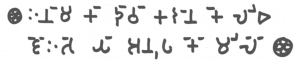
\includegraphics[scale=1.5]{content/fmatter/easteregg.pdf}

\vspace{1.0em}
\noindent ACL 2018 Program Committee Co-Chairs \\
Iryna Gurevych, TU Darmstadt, Germany \\
Yusuke Miyao, National Institute of Informatics, Japan
\index{Gurevych, Iryna}
\index{Miyao, Yusuke}
